\documentclass[a4paper,twoside]{report}
\usepackage{graphicx}
\usepackage{dsfont}
\usepackage{epsf,amsthm,amsmath}
\usepackage[ngerman]{babel}
\usepackage[latin1]{inputenc}
\usepackage{graphicx}
\setlength{\parskip}{5pt plus 8pt minus 2pt}
\pagestyle{headings}

\begin{document}
\begin{titlepage}
\ \vfill
\Large
\begin{center}
{\LARGE\bf Proseminar} \\[1cm]
{\huge\bf Stochastische Dynamische Optimierung\par}
\vspace*{1cm}
\input unilogo
\unilogo{30}\\[1cm]
{\bf Universit"at Karlsruhe (TH)}\\
{Fakult"at f"ur Mathematik}\\
{\em Institut f"ur Mathematische Stochastik}
\vfill
Priv.-Doz.~Dr.~D.~Kadelka\\
Dr.~B.~Klar
\vfill\vfill 
Sommersemester 2004
\vfill
\vfill
\end{center}
\end{titlepage} 
\thispagestyle{empty}
\ 
\vfill
\noindent
Copyright $\copyright$ 2004\\
Institut f"ur Mathematische Stochastik\\
Fakult"at f"ur Mathematik\\
Universit"at Karlsruhe\\
Englerstra"se 2\\
76\,128 Karlsruhe


\title{Stochastic Scheduling}
\author{Clemens Lode}
\date{}
\maketitle

\pagenumbering{roman}
\tableofcontents

\pagenumbering{arabic}

\setcounter{chapter}{2}
\chapter{Stochastic scheduling}
\section{Einleitung}

\textsc{Stochastic Scheduling} besch"aftigt sich mit Problemen, bei denen die Laufzeiten eines Jobs durch Zufallsvariablen dargestellt sind. Dadurch ist die tats"achliche Zeit vor Ende des Jobs unbekannt. Das 'Scheduling' ist je nach Problem auf ein oder mehrere Prozessoren und mit verschiedenartigen Nebenbedingungen best"uckt.

Hier im Speziellen m"ochte ich auf 4 Probleme aus diesem Bereich eingehen die mit der Abarbeitung von Jobs auf ein oder mehreren Prozessoren zu tun haben. Dabei ben"otigt jeder Job eine gewisse Zeit \(X_{j}\), die eine exponentiale Verteilung besitzt. 

\section{Fall: Ein Prozessor}

Zum Einstieg ein triviales Problem um mit den verwendeten Variablen und ein paar einfachen Gesetzm"assigkeiten im weiteren Verlauf besser zurechtzukommen. 
Das Problem in diesem Fall ist, dass wir n Jobs auszuf"uhren haben. Ein Job ist dabei eine beliebige Aufgabe die ein Prozessor berechnen kann, der eine bestimmte Zeit braucht, wobei die Jobs nicht gleich sein m"ussen.
Au"serdem haben wir im ersten Fall einen einzelnen Prozessor zur Verf"ugung, der immer nur einen Job gleichzeitig bearbeiten kann. Die Fragestellung ist nun, welche Reihenfolge der Jobs, im Folgenden Politik genannt, die Zeit um alle Jobs auszuf"uhren minimiert.

Was ist die ben"otigte Gesamtzeit unserer Jobs? Bei einem realistischen Beispiel w"are das schwer zu sagen. Verbraucht z.B. ein Job w"ahrend und nach der Bearbeitung sehr viel Speicher w"are wohl das Beste diesen hinten hinzustellen, damit die anderen Jobs nicht z.B. auf der langsamen Festplatte ausgelagert werden m"ussen. Die Zeit die ein einzelner Job ben"otigt w"are also vom bisherigen Verlauf abh"angig.

Wir machen es uns jedoch einfach und begrenzen uns auf den Fall, dass \emph{alle Jobs unabh"angig voneinander} bearbeitet werden k"onnen. Dies bedeutet, die einzelnen Jobs sind \emph{ged"achtnislos}, d.h. in diesem Fall, dass zu jedem Zeitpunkt t auf Basis der bisherigen Ereignisse die bedingte Wahrscheinlichkeit fuer jeden neuen Job eine bestimmte Zeit zu brauchen genau so gro"s ist, als w"are dies der erste Job in der Auftragsliste.

Im weiteren werde ich folgende Definitionen und Voraussetzungen gebrauchen:
\begin{itemize}
\item M: ben"otigte Gesamtzeit bis alle Jobs abgearbeitet sind
\item Politik \begin{displaymath}\pi = (i_{1},i_{2},\ldots,i_{n})\end{displaymath} wobei \(i_{j}\) \(\neq\) \(i_{k}\) f"ur \(j \neq k\) und \(0<i_{j}\le n\) eine Jobnummer bezeichnet.
\item \(X_{j}\) ist eine exponential verteilte Zufallsvariable mit Parameter \begin{displaymath}\lambda_{j} = \frac{1}{u_{j}}\end{displaymath}
\item \(u_{j}\) entspricht somit der erwarteten Zeit die Job \(X_{j}\) ben"otigt
\end{itemize}
Im Weiteren gehen wir au"serdem davon aus, dass zum Zeitpunkt 0 bereits ein Job 0 auf dem Prozessor liegt.

Die Gesamtzeit unserer Jobs ist dann nat"urlich die Summe aller Zeiten und somit von der Reihenfolge unabh"angig. Also ist es, wie man es erwartet h"atte, vollkommen egal, welche Politik man w"ahlt. F"ur die erwartete Gesamtzeit ergibt sich also:

\begin{displaymath} E(M) = E(X_{i_{1}})+E(X_{i_{2}})+\cdots+E(X_{i_{n}}) = \sum_{j=1}^{n} E(X_{j})\end{displaymath}

wobei die Summe unabh"angig von den \(i_{j}\), also der Reihenfolge der Jobs, ist.

\begin{figure}[h]
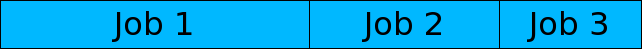
\includegraphics[scale=0.5]{durchlaufpolitik1.png}
\caption{M"oglicher Durchlauf bei gegebener Politik \(\pi_{1} = (1,2,3)\)}
\end{figure}

\begin{figure}[h]
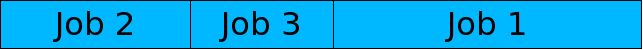
\includegraphics[scale=0.5]{durchlaufpolitik2.png}
\caption{Der selbe Durchlauf mit anderer Politik \(\pi_{2} = (2,3,1)\)}
\end{figure}

Mit dieser kleinen Einf"uhrung k"onnen wir uns nun an ein schwierigeres Problem wagen, wir legen im zweiten Teil einen weiteren Prozessor hinzu.

\newpage\section{Fall: Zwei Prozessoren parallel}

\subsection{Problemdefinition und Ansatz}

Es sind wieder eine Reihe von Jobs gegeben, die unterschiedlich lange Zeit ben"otigen. Au"serdem hat man ein System mit diesmal zwei identische Prozessoren zur Verf"ugung. Die einzelnen Jobs sind stochastisch unabh"angig und exponential verteilt. Das Problem ist nun wieder, eine Politik f"ur die Abarbeitung der Jobs zu finden, so dass die insgesamt ben"otigte Zeit minimal ist.

\begin{figure}[h]
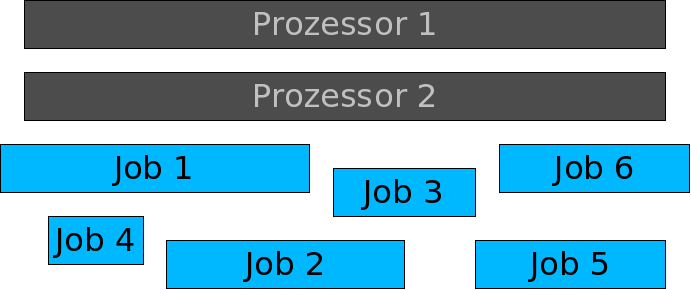
\includegraphics[scale=0.5]{zweiprozessoren.png}
\caption{"Ubersicht Problemstellung zwei Prozessoren - mehrere Jobs m"ussen auf 2 Prozessoren verteilt werden}
\end{figure}

Ein erster Ansatz w"are, die Politiken so aufzubauen, dass wir jedem Job j einen Zeitpunkt k und einen Prozessor l zuordnen. Zwar sind damit alle m"oglichen Kombinationen abgedeckt, jedoch ergibt sich beim Zeitpunkt k ein Problem: Es ergeben sich einerseits Zeiten in der Prozessoren ungenutzt sind (siehe Abb. 3.4), die deshalb auftreten, weil die Ausf"uhrungszeiten \(X_{j}\) der Jobs zu Beginn unbekannt sind. Andererseits gibt es keine festen Zeiteinheiten auf die wir unsere Jobs verteilen k"onnten was zu unendlich vielen M"oglichkeiten f"uhren w"urde. Vor allem auf Grund der ungenutzten Zeiten bei dieser Art von Politik kann in diesem Fall die optimale L"osung f"ur die gegebenen Voraussetzungen nicht gefunden werden.

\begin{figure}[h]
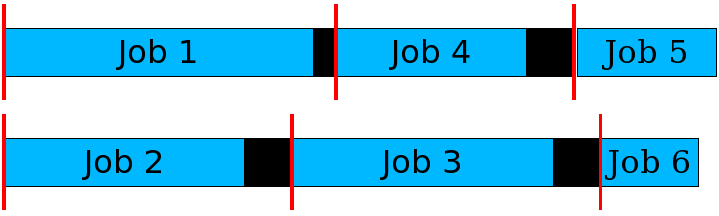
\includegraphics[scale=0.5]{zeitzuordnung2.png}
\caption{Zustand Prozessoren mit Politik die nach Zeit zuordnet - schwarz markierte Bereiche geben ungenutzte Zeiten des Prozessors an}
\end{figure}

Die Einteilung nach den Zeitpunkten k"onnen wir umgehen indem wir eine Voraussetzung, sogenanntes \emph{Expertenwissen}, f"ur unser Problem benutzen. Wir m"ussen n"amlich "uber die genaue Positionen der Jobs zu Beginn noch nichts wissen, wir k"onnen uns entscheiden welchen Job wir als n"achstes einf"ugen sobald einer der beiden Prozessoren frei wird, was auch zur Schlie"sung der L"ucken f"uhrt.

Der zweite Versuch eine Politik aufzustellen, w"are also, dass man jeden Job in eine der zwei Reihen in einer bestimmten Reihenfolge einf"ugt. Wir ordnen also jedem der n Jobs einen Prozessor zu (\(2^{n}\) M"oglichkeiten) und legen die Reihenfolge der n Jobs fest (n * (n-1) * \(\ldots\) * 2 * 1 = n! M"oglichkeiten) wodurch sich insgesamt \(2^{n} n!\) verschiedene Belegungen f"ur die Politik ergibt.


\subsection{Zu minimierende Zielfunktion} ~~~

Seien zwei identische Prozessoren gegeben um n Jobs abzuarbeiten. Beide laufen unabh"angig, k"onnen also jede Aufgabe zu jeder Zeit in einer beliebigen Reihenfolge bearbeiten. Startzeit ist t = 0. Sei au"serdem \(X_{j}\) die Zeit um Aufgabe j zu bearbeiten und sei diese exponential verteilt mit \begin{displaymath}\lambda_{j} = u_{j}, j=1,\ldots,n\end{displaymath}.

F"ur jede Politik \(\pi\) ist jeweils M die Bearbeitungsdauer und D die Zeit die einer der Prozessoren stillsteht. Somit ist zum Zeitpunkt M - D einer der Prozessoren fertig und keine weiteren Auftr"age mehr in der Warteschlange und M + M - D ist die Summe aller Zeiten, also \(\sum_{j=0}^n X_{j}\)

Also gilt: \(2M - D - \sum_{j=0}^{n} X_{j} = 0\) und somit f"ur jede Politik \(\pi\):

\begin{displaymath}E_{\pi}(2M-D-\sum_{j=0}^{n} X_{j}) = E_{\pi}(0)\end{displaymath}

\begin{displaymath}2* E_{\pi} (M) = E_{\pi} (D) + \sum_{j=0}^{n} E_{\pi} (X_{j})\end{displaymath}

Da nach Voraussetzung die \(X_{j}\) von einander also insbesondere auch von der Wahl der Politik \(\pi\), unabh"angig sind, ist \(\sum_{j=0}^{n} E(X_{j})\) eine Konstante f"ur jede Politik \(\pi\) (f"ur die gleichen \(X_{j}\)) und wir setzen \(c = \sum_{j=0}^{n} E(X_{j})\):

\begin{equation}\label{e31}E_{\pi}(M) = \frac{E_{\pi}(D) + c}{2}\end{equation}

Also ergibt sich, dass durch Minimierung der erwarteten Differenz D in der einer der Prozessoren unbesch"aftigt ist, auch die Bearbeitungsdauer minimiert wird.

\subsection{Verfeinerung der Politik}
	
Zwar k"onnte man unter Umst"anden auch mit dem Modell jedem Job einen Prozessor zuzuordnen auf die einzelnen Aussagen und S"atze kommen, jedoch ist es bei Optimierungsaufgaben grunds"atzlich hilfreich, die Zahl der unterschiedlichen Politiken so weit wie m"oglich zu verringern. Dabei ist nat"urlich immer darauf zu achten, dass der optimale Fall mit der Politik noch herzustellen ist.

\textbf{Behauptung}: Eine Politik f"ur den Fall mit zwei Prozessoren die die Jobs nach ihrer Reihenfolge immer auf den Prozessor legt, der gerade frei ist, ist gleichwertig mit einer Politik die jedem Job zus"atzlich einen beliebigen Prozessor zuweist.

Mit ''gleichwertig'' ist gemeint, dass mit beiden Politiken die Jobs so verteilt werden k"onnen, dass die insgesamte ben"otigte Zeit bei beiden Politiken gleich und minimal ist.

\textbf{Beweisidee}: Es ist klar, dass der Versuch auf den einen Prozessor alle Jobs und auf den anderen Prozessor keine Jobs zu verteilen f"ur \(n>1\) nicht zum optimalen Ergebnis f"uhrt, da die erwartete Differenz D in dem Fall maximal w"are. So eine 'kaputte' Politik k"onnte man aber 'reparieren' in dem man, zu jedem Zeitpunkt bei einer der beiden Prozessoren keine Aufgabe zu bearbeiten hat, einfach die n"achste Aufgabe aus unserer Politik zuweisen. 

Jede Politik die mit der Konstruktionsmethode aus der Behauptung nicht hergestellt werden kann, kann keine optimale Politik sein~~, da


G"abe es zu irgendeinem Zeitpunkt 

Wenden wir diese Regel auf jede unserer Politiken an, folgt, dass eine Politik die alle n Jobs auf einen Prozessor legt, \emph{gleichwertig} zu allen anderen Kombinationen der Verteilung der Jobs ist. 

%\begin{figure}[h]
%\includegraphics[scale=0.5]{zweiprozessorenpfeile.png}
%\caption{Zwei Prozessoren - eine Politik}
%\end{figure}

Dies reduziert unseren Zahl unterschiedlicher Politiken auf \textbf{n!} und erleichtert die folgenden Beweise, da wir nur noch Politiken haben, die aus \emph{einer} anstatt zwei Reihen von Jobs bestehen. Wir k"onnen uns nun dem eigentlichen Problem widmen:

Die Frage ist nun zuerst, ob durch unsere Regel das Problem nicht schon gel"ost wurde. Wenn wir immer eine Aufgabe auf den Prozessor legen, der nicht besch"aftigt ist, gleichen wir bei jedem Schritt beide Balken aus. Erreichen wir dadurch das optimale Gleichgewicht? Nein. Dies w"urde der Fall sein, wenn alle Jobs gleiche Zeit ben"otigten und eine gerade Anzahl Jobs vorliegt. Legen wir aber beispielsweise die Jobs mit aufsteigenden Zeiten auf die Prozessoren, schwankt der Unterschied zwischen beiden bei jedem Schritt mehr, 
	
\begin{tabular}{|r|ccc|}
\hline
Schritt & Idle-Zeit & 1. Prozessor & 2. Prozessor \\
\hline
0 & 1 & 1 & 0 \\
1 & 1 & 1 & 2 \\
2 & 2 & 4 & 2 \\
3 & 2 & 4 & 6 \\
4 & 3 & 9 & 6 \\
5 & 3 & 9 & 12 \\
... & ... & ... & ... \\
\hline
\end{tabular}

%\caption{Idlezeit bei aufsteigender Sortierung}

%Dass dies auch wirklich ein Problem darstellt, die Gesamtzeit also von der Reihenfolge abh"angt, macht dieses Beispiel schnell klar:
%Angenommen wir h"atten 5 Jobs mit den Zeiten 10, 8, 12, 5 und 1. Legen wir sie nun auf die 2 Prozessoren:

%P1 |||||||||#||||##
%P2 |||||||#|||||||||||#

%Man sieht also, dass mit dieser Reihenfolge ein Prozessor 4 Zeiteinheiten unbesch"aftigt ist. 
%Auch wird klar, dass egal wie wir es anstellen, die untere Schranke f"ur die ben"otigte Zeit (10 + 8 + 12 + 5 + 1) / 2 ist, wenn also beide Prozessoren bis zum Ende voll besch"aftigt sind.

Investiert man in die Aufgabe etwas Denkarbeit wird auch klar, dass wohl die optimale Politik w"are, wenn wir grunds"atzlich mit den l"angsten Jobs beginnen und am Schluss die k"urzesten Jobs legen. Warum? Weil wir bei jedem Schritt die Aufgabe grunds"atzlich nur auf den Prozessor legen, der gerade frei ist. Wir versuchen also bereits dadurch die beiden Balken auszugleichen. Je sp"ater wir eine l"angere Aufgabe auf einen Prozessor legen, desto unwahrscheinlicher k"onnen wir diesen mit den restlichen Jobs wieder ausgleichen.

\subsection{Erster Beweisschritt: Vergleich zweier Politiken}

Sei im weiteren Verlauf zum Zeitpunkt 0 ein Job 0 bereits im Prozessor, d.h. starte jede Politik mit Job 0 (dies macht den Beweis etwas klarer).

Als n"achstes wird gezeigt, dass eine Politik die in aufsteigender Reihenfolge der \(u_{i}\) (also der absteigenden Zeiten) angeordnet ist, optimal ist. Dazu betrachten wir zwei nahezu gleiche Politiken, bei der Job 1 und Job 2 miteinander vertauscht sind und beweisen dann induktiv:

\textbf{Lemma 1:} Seien zwei Politiken \(\pi\) und \(\bar \pi\) gegeben:
\begin{displaymath}\pi = (0,2,1, i_{3}, i_{4},\ldots,i_{n})\end{displaymath} 
\begin{displaymath}\bar \pi = (0, 1,2,i_{3}, i_{4},\ldots,i_{n})\end{displaymath} 
Gelte au"serdem, dass \(u_{1} = min_{k \ge 1}(u_{k})\), dann gilt:
\begin{displaymath}E_{\bar \pi}(D)\le E_{\pi}(D)\end{displaymath}.


\textbf{Beweis:} Seien \(p_{j}\) und \(\bar p_{j}\), j \(\ge\) 0 die zu \(\pi\) und \(\bar\pi\) geh"origen Wahrscheinlichkeiten, dass die letzte von den Prozessoren abgeschlossene Aufgabe Job j ist, also z.B. Prozessor A fertig ist und Prozessor B noch an Aufgabe j arbeitet und keine weiteren Jobs mehr in der Warteschlange/Politik liegen.

\begin{displaymath}p_{0} = \bar p_{0} = P(X_{0} > \sum_{j=1}^{n} X_{j})\end{displaymath} ist klar. Der erste Job entspricht der Wahrscheinlichkeit, dass \(X_{0}\) gr"osser ist als alle anderen zusammengenommen, da \(p_{0}\) ja jeweils der erste Job in beiden Politiken \(\pi\) und \(\bar \pi\) ist.

Wir wollen nun durch Induktion zeigen, dass \begin{equation}\label{e32}\bar p_{1} \le p_{1}, \qquad \bar p_{j} \ge p_{j}, \qquad  j=2,\ldots,n\end{equation}

\textbf{Induktionsanfang:} F"ur n = 1 f"allt \(\bar p_{j} \ge p_{j}\) f"ur j = 2,\ldots,n sowieso weg, da \(n < 2\) und \(\bar p_{1} \le p_{1}\) gilt nach der Voraussetzung \(u_{1}\) = \(min_{k \ge 1}(u_{k})\), da \(\pi\) an der Stelle 1 \(u_{1}\) stehen hat und \(\bar \pi\) dagegen \(u_{2}\).

\textbf{Induktionsvoraussetzung:} Es gelte also die Behauptung (\ref{e32}) f"ur den Fall, dass nur n-1 Jobs (zus"atzlich zu Job 0) vorliegen und somit:
\begin{equation}\label{e33}\bar p_{1}^{*} \le  p_{1}^{*}, \qquad \bar p_{j}^{*} \ge  p_{j}^{*}, \qquad  j=2,\ldots,n-1\end{equation}

\textbf{Induktionsschluss:} Seien nun diesmal (n-1)+1 = n Jobs zu erledigen und seien \( p_{j}^{*}\) und \(\bar p_{j}^{*}\) (wieder zugeh"orig zu \(\pi\) und \(\bar\pi\), j=1,\ldots,n-1) die Wahrscheinlichkeiten, dass Job j der letzte der Jobs 0,\ldots,n-1 f"ur die jeweilige Politik ist.
Da die Jobs unab"angig sind, k"onnen wir zur Betrachtung des letzten Jobs alle vorherigen abgeschlossenen Jobs ignorieren, diese haben keine Auswirkung auf die Bearbeitungszeit f"ur den letzten Job. Allerdings liegt unter Umst"anden auf dem anderen Prozessor noch ein letzter Job n der zu Beginn des letzten Jobs noch nicht abgeschlossen ist. Nach der Ged"achtnislosigkeit l"auft dieser Job n noch \(X_n\) Zeiteinheiten obwohl er schon einige Zeit gelaufen ist.
Daraus folgt, dass die Wahrscheinlichkeit, dass Job j und nicht Job n der letzte bearbeitete Job ist, P(\(X_{j} > X_{n}\)) entspricht:

\begin{displaymath}P(X_{j} > X_{n}) = P(X_{n} < x | X_{j} = x) = \int_{0}^{\infty}(1 - e^{-\lambda_{n}x})\lambda_{j}e^{-\lambda_{n}x} dy\end{displaymath}
\begin{displaymath}= \int_{0}^{\infty} (\lambda_{j}e^{-\lambda_{j}x} - \lambda_{j}e^{(-\lambda_{n}-\lambda_{j})x})dy = [-e^{-\lambda_{j}x} + \frac{\lambda_{j}}{\lambda_{j}+\lambda_{n}} e^{(-\lambda_{n} - \lambda_{j})x}]_{0}^{\infty}\end{displaymath}
\begin{displaymath}= 1 - \frac{\lambda_{j}} {\lambda_{j} + \lambda_{n}} = \frac{ \frac{1}{u_{n}} }{ \frac{1}{u_{j} } + \frac{1}{u_{n}}} = \frac{u_{n}}{u_{j} + u_{n}}\end{displaymath}

Da diese Wahrscheinlichkeit unabh"angig von der Wahrscheinlichkeit ist, dass j der letzte Job ist im Fall mit insgesamt (n-1) Jobs ist, k"onnen wir die Gesamtwahrscheinlichkeit durch einfache Multiplikation berechnen:

\begin{displaymath}p_{j} =  p_{j}^{*} P(X_{j} > X_{n}) = p_{j}^{*} \frac{u_{n}}{u_{n} + u_{j}}, \qquad \bar p_{j} = \bar p_{j}^{*} P(X_{j} > X_{n}) = \bar p_{j}^{*} \frac{u_{n}}{u_{n} + u_{j}}, \qquad j = 1,\ldots,n-1\end{displaymath}

Daraus und aus (\ref{e33}) folgt, dass
\begin{equation}\label{e34}\bar p_{1} \le p_{1}, \qquad \bar p_{j} \ge p_{j}, \qquad j=2,\ldots,n-1\end{equation}

%\begin{figure}[h]
%\includegraphics[scale=0.5]{gedlosigkeitabschneiden.png}
%\caption{Abschneiden unter Ausnutzung der Ged"achtnislosigkeit}
%\end{figure}

%|||||||||| (n-4) ||||||||| (n-2) ||| (n-1) ||||||||||| (n)
%|||||||||||||||||| (n-3) ||||||||||||||||||| (j = n-2)

Um nun auch \(p_{n}\) und \(\bar p_{n}\) vergleichen zu k"onnen benutzen wir die Gegenwahrscheinlichkeit und bilden die Differenz:

\begin{displaymath}\bar p_{n} - p_{n} =  \sum_{j=0}^{n-1}(\bar p_{j} - p_{j}) = \sum_{j=0}^{n-1}(( p_{j}^{*} - \bar p_{j}^{*}) \frac{u_{n}}{u_{n} + u_{j}} =\end{displaymath}
Durch Abspalten des ersten Gliedes ergibt sich:
\begin{displaymath}=( \bar p_{1}^{*} -  p_{1}^{*}) \frac{u_{1}}{u_{1} + u_{n}} + \sum_{j=2}^{n-1} (\bar p_{j}^{*} -  p_{j}^{*}) \frac{u_{j}}{u_{j}+u_{n}} \end{displaymath}
Dies k"onnen wir mit Hilfe von \(u_{j} \ge u_{1} \Leftrightarrow \frac{u_{j}}{u_{j} + u_{n}} \ge \frac{u_{1}}{u_{1} + u_{n}}\) absch"atzen:
\begin{displaymath}\ge \frac{u_{1}}{u_{1}+u_{n}} \sum_{j=1}^{n-1} (\bar p_{j}^{*} -  p_{j}^{*}) = 0\end{displaymath}

Aus \(\bar p_{n} \ge p_{n}\) und (\ref{e34}) folgt nun die Behauptung (\ref{e32}) und wir haben das Lemma 1 bewiesen.



\subsection{Zweiter Beweisschritt: allgemeiner Fall}

\textbf{Korollar 1:} Lemma 1 gilt auch f"ur beliebige Politiken der Form \(\pi = (0, 1, i_{2}, i_{3}, \ldots, i_{n})\) und \(\bar \pi = (0, i_{2}, 1, i_{3} \ldots, i_{n})\) mit \(u_{i_{2}} \ge u_{1}\).

\textbf{Beweis:} Da wir zum Beweis von Lemma 1 nur \(u_{j} \ge u_{1}\) benutzt haben und nicht direkt verwendet haben, dass \(i_{2} = 2\) gelten muss, gilt das Korollar 1.

\textbf{Lemma 2:} Seien zwei Politiken \(\pi\) und \(\bar \pi\) gegeben:
\begin{displaymath}\pi  = (0,i_{1},i_{2},\ldots,i_{k-2},i_{k-1}=1,i_{k},i_{k+1},\ldots,i_{n})\end{displaymath}
\begin{displaymath}\bar\pi = (0, i_{1}, i_{2},\ldots, i_{k-2}, i_{k}, i_{k-1}=1, i_{k+1},\ldots, i_{n})\end{displaymath}
Gelte au"serdem, dass \(u_{1} \le u_{2} \le \ldots \le u_{n}\), dann gilt:
\begin{displaymath}E_{\bar \pi}(D)\le E_{\pi}(D)\end{displaymath}.

\textbf{Beweis:} Da die Jobs hier wiederum unbabh"angig voneinander sind, haben Job 0 bis \(i_{k-2}\) keinen Einfluss auf die Nachfolgenden, wie auch \(i_{k-1}\) und \(i_{k}\) keinen Einfluss auf die Zeiten der nachfolgenden Jobs haben. Somit kann man diese zu einem neuen Job \(\bar 0\) zusammenfassen und es ergibt sich "aequivalente Politiken:

\begin{displaymath}\pi = (\bar 0, 1 ,i_{k}, i_{k+1}, \ldots, i_{n}), \qquad \bar\pi = (0, i_{k},1, i_{k+1}, \ldots, i_{n})\end{displaymath}

Nach Korollar 1 folgt nun, da \(u_{1} = min_{k \ge 2}(u_{k})\), direkt Lemma 2.

\textbf{Korollar 2:} Lemma 2 gilt auch f"ur beliebige Jobs j sofern alle \(u_{i_{k}} \ge u_{j}\) mit \(i_{k} > j\) und alle \(u_{i_{k}} \le u_{j}\) mit \(i_{k} < j\), der Job j also genau der Job mit der niedrigsten Nummer ist, der bisher noch nicht betrachtet wurde.

\textbf{Beweis:} Durch Vertauschen mit Jobs niedriger Nummer k"onnen wir den Erwartungswert f"ur D nicht verringern, da nach Voraussetzung alle \(u_{i_{k}}\) kleiner sind als \(u_{j}\). Wir d"urfen also wie bei Lemma 2 die bisherigen Jobs zu einem Job \(\bar 0\) zusammenfassen. In dieser neuen "aquivalenten Politik ist der Job j nun wieder insgesamt der Job mit dem kleinsten Wert \(u_{j}\), somit gilt wie Korollar 1 auch Korollar 2.

TODO \(<\) UND \(>\) PRUEFEN

\textbf{Satz 1:} Eine aufsteigend sortierte Politik \(\pi = (0,1,2,\ldots,n)\) ist die optimale Politik um den Erwartungswert f"ur D zu minimieren, falls \(u_{1} \le u_{2} \le \ldots \le u_{n}\) gilt.

\textbf{Beweis:} Durch mehrmaliges Anwenden von Lemma 2 und Korollar 2 (mit Job 2, Job 3 usw.) erreichen wir eine aufsteigende Reihenfolge, wobei bei jeder Iteration der Erwartungswert fuer die Zeit die ein Prozessor nichts zu tun hat (D) weiter sinkt bzw. gleich bleibt. Ist die aufsteigende Reihenfolge erreicht gibt es keine M"oglichkeit den Erwartungswert f"ur D weiter zu senken. Somit ist 

TODO IST DAS AUCH GLOBALES OPTIMUM?

\newpage
\section{Ein Prozessor mit begrenzter Zeit}

Mit diesem Problembeispiel m"ochte ich auf einen weiteren Aspekt des \textsc{Stochastic Scheduling} eingehen. Wir haben wie vorher auch n Jobs die ausgef"uhrt werden sollen, haben diesmal aber eine \emph{feste Zeitbegrenzung t}, die wahrscheinlich dazu f"uhrt, dass nicht alle Jobs ausgef"uhrt werden k"onnen.
Der Unterschied zum ersten Beispiel ist nun aber, dass wir jedem Job i eine Priorit"at \(R_{i}\) zuordnen und die Qualit"at einer Politik nicht wie vorher "uber die Zeit sondern "uber die Summe der Priorit"aten bestimmen, es soll also \begin{displaymath}E(Gewinn) = \sum_{i=0}^{n} ER_{i}(s_{i})\end{displaymath} maximiert werden, wobei \(s_{i} = 1\) ist, wenn der Job ausgef"uhrt werden konnte und 0 wenn nicht.
Auch hier gilt wieder die Unabhaengigkeit der Ausf"uhrungszeiten der Jobs. Wenn also bereits \(1 - t_{i}\) Zeiteinheiten durch andere Jobs verstrichen sind, k"onnen wir den n"achsten Job i als den ersten Job einer Politik zu dem Problem bei der noch \(t_{i}\) Zeiteinheiten "ubrig sind.

Wir schreiben die \(s_{i}\) als Wahrscheinlichkeiten aus um es mit dem Erwartungswert benutzen zu k"onnen. Die Wahrscheinlichkeit, dass Job i ausgef"uhrt wird ist und noch \(t_{i}\) Zeiteinheiten "ubrig sind, betr"agt wegen Exponentialverteilung:
\begin{displaymath} s_{i} = P(X_{i} < t_{i}) = 1 - e^{-\lambda_{i}t_{i}}\end{displaymath}

Das \(t_{i}\) ist nat"urlich abh"angig von den fr"uheren Jobs. Da wir uns f"ur einen neuen Job jedoch immer erst entscheiden, wenn ein Prozessor frei ist, kennen wir zu diesem Zeitpunkt \(t_{i}\) und k"onnen es als Konstante benutzen.

Somit ergibt sich f"ur den erwarteten Gewinn f"ur einen Job i und verbleibender (konstanter) Zeit \(t_{i}\):

\begin{displaymath} R_{i} P(X_{i} < t_{i}) = R_{i} (1-e^{-\lambda_{i} t_{i}}) = \lambda_{i} R_{i} \frac{1-e^{-\lambda_{i} t_{i}}}{\lambda_{i}} \end{displaymath}
\begin{displaymath} = \lambda_{i} R_{i} E[min(X_{i}, t_{i})] \end{displaymath}

Die letzte Gleichheit folgt aus:

\begin{displaymath} E[min(X_{i}, t_{i})] = \int_{0}^{\infty} P[min(X_{i}, t_{i}) > x] dx\end{displaymath}
\begin{displaymath} = \int_{0}^{t_{i}} e^{-\lambda_{i}x} dx = \frac{(1- e^{-\lambda_{i} t_{i}})}{\lambda_{i}}\end{displaymath}

\(min(X_{i}, t_{i})\) entspricht dabei der Zeit, die der Prozessor an diesem Job i noch arbeitet, ob er abgebrochen wird oder nicht.

Den Gesamtgewinn haben wir oben bereits definiert, wir m"ussen nur noch unser Ergebnis einsetzen:

\(E_{\pi} (Gesamtgewinn) = \sum_{i=0}^{n} \lambda_{i} R_{i} E_{\pi}( min(X_{i}, t_{i}) )\)


Bleibt die Frage offen, was \(t_{i}\) in diesem Zusammenhang bedeutet. F"ur einen einzelnen Job konnten wir J festsetzen


Zwar ist die Politik \(\pi\) eine station"are Politik, die Reihenfolge der Jobs wird zu Beginn festgelegt, wann und auf welchen Prozessor die Jobs jedoch eingesetzt werden wird w"ahrend der Abarbeitung der Politik festgelegt. 

Zwar k"onnte man mit gro"sem Aufwand den Erwartungswert von \(t_{i}\) "uber die Politik und die vor Job i stehenden \(X_{j}\) berechnen, um die optimale Politik zu finden und dann wie im vorherigen Kapitel zwei Politiken vergleichen und dann mit Induktion die Optimalit"at einer bestimmten Reihenfolge , reicht es zu wissen, ben"otigen wir jedoch nicht den Erwartungswert an sich sondern 


Zwar ist 

Um den Wert \(t_{i}\) zu kennen, muss man die 

TODO WARUM FOLGT \(\lambda_{i} R_{i}\)

Also folgt:

\textbf{Satz 2:} Der Gesamtgewinn bei gegebener Zeit t wird maximiert, wenn eine Politik gew"ahlt wird, die die Jobs in einer absteigenden Folge von \(\lambda_{i} R_{i}\) f"ur i=1,\ldots,n.
 

\newpage
\section{Zwei Prozessoren mit begrenzter Zeit TODO}

Im letzten Teil kombinieren wir nun die vorherigen zwei Problemstellungen. Wir haben zwei Prozessoren, eine feste Zeit t und f"ur jeden Job eine Priorit"at \(R_{j}\).
Nach 2.1 ist der Gesamtgewinn ~~ unter einer Politik \(\pi\):
\(E_{\pi}\)(Gesamtgewinn abh"angig von t) = \begin{displaymath}\sum_{j=0}^{n} u_{j}R_{j}E_{\pi}\end{displaymath}(Verarbeitungszeit von Job j nach t ~~)

Es sieht nun so aus, als ob wir hier wie in 2.1, der Fall bei dem wir nur ein Prozessor zur Verf"ugung hatten, die optimale Politik eine absteigende Reihenfolge der \(u_{j}\)\(R_{j}\) ist, also wir Jobs um so weiter hinten positionieren je gr"o"ser die erwartete ben"otigte Zeit und je kleiner die Priorit"at ist.

Dies ist aber nicht der Fall wie ein kleines Gegenbeispiel zeigt:

\(u_{j}\)\(R_{j} \equiv 1\) f"ur alle j und \begin{displaymath}u_{1} < u_{2} < \cdots < u_{n}\end{displaymath}.

Es w"urde folgen, dass, da ja alle \(u_{j}\)\(R_{j}\) gleich gro"s sind, jede beliebige Reihenfolge optimal ist. Dies stimmt auch im Fall von einem Prozessor, bei zwei Prozessoren tritt jedoch wie anfangs besprochen eine immer gr"o"sere Idle Zeit auf, wenn wir die Jobs absteigend nach den \(u_{j}\) (bzw. aufsteigend nach den ben"otigten Zeiten) sortieren.

Wir k"onnen jedoch zeigen, dass wie im Fall ohne Priorit"aten eine aufsteigende Reihenfolge optimal ist, wenn wir gewisse Bedingungen voraussetzen.

\textbf{Behauptung:}
Sei 
\begin{displaymath}u_{1} \le u_{2} \le \cdots \le u_{n}\end{displaymath} 
und 
\begin{displaymath}u_{1}R_{1} \ge u_{2}R_{2} \ge \cdots \ge u_{n}R_{n} \ge 0\end{displaymath}
dann ist die Reihenfolge (1, 2, \ldots, n) optimal und maximiert den zu erwartenden Gesamtgewinn f"ur Zeit \(t>0\).

\textbf{Beweis:}

Wir benutzen hierzu die aus dem vorherigen Kapitel bekannten Zeiten die ein Job noch ben"otigt \(T_{i} = min(X_{i}, t_{i})\) und setzen \(c(i) = u_{i}R_{i}\), sodass nach Voraussetzung gilt: \(c(1) \ge c(2) \ge c(3) \ge \ldots c(n) \ge 0\).
TODO

\newpage
\section{Ausblick und Zusammenfassung}

Insgesamt hat dieser Vortrag zeigen k"onnen, wie man sich Schritt f"ur Schritt an eine Problemstellung des Stochastic Scheduling herann"ahert und dann durch Benutzung der Voraussetzungen, hier vor allem der Ged"achtnislosigkeit und der Induktion, die einzelnen Aussagen zu beweisen.

In den ersten zwei Kapiteln wurde neben einigen Definitionen vor allem auf die Herangehensweise wert gelegt, wie also eine Politik zu definieren ist. Au"serdem wurde gezeigt, dass es f"ur das jeweilige Problem unterschiedlich gut angepasste Politiken gibt. Hier wurde ein Vergleich der Politik 'Setze Jobs an bestimmten Zeiten' und der Politik 'Setze Jobs sobald der Prozessor frei wird' aufgestellt, der gezeigt hat, dass durch Einbringen von genauer Kenntnis des Problems die Politik wesentlich vereinfacht werden konnte, ohne dass der optimale Fall verloren geht.

Im ersten Kapitel wurde auf den Problemfall mit einem einzelnen Prozessor eingegangen. Mit korrekter Politikdefinition lie"s sich das Problem relativ trivial l"osen, alle Politiken waren optimal, da \(E(\sum_{j=0}^{n} X_{i_{j}})\) von der Anordnung der Jobs \(i_{j}\) unabh"angig war. 
			
Das Kapitel hat den Weg fuer das zweite Kapitel geebnet, bei dem wir auf den Fall mit zwei Prozessoren eingegangen sind. Auch hier wurde die Politikdefinition selbst erst auf die Problemstellung definiert, in dem nicht f"ur jeweils einen Prozessor eine seperate Politik definiert wurde, sondern durch intelligente Wahl der Einf"ugeregel wir uns wieder auf eine Politik beschr"anken konnten ohne dabei den optimalen Fall zu verlieren. Das Ergebnis hier war interessanter, eine Anordnung der Jobs nach absteigendem \(u_{j}\) war optimal, was einerseits bildlich anhand von Balkengrafiken gezeigt wurde, andererseits mit Hilfe von Induktion und der Ged"achtnislosigkeit bewiesen wurde.

Im dritten Kapitel sind wir wieder auf den Fall mit einem Prozessor zur"uckgekehrt und haben den Fall mit begrenzter Zeit und entsprechender Entlohnung bei Fertigstellung des entsprechenden Jobs betrachtet. Im Beweis f"ur die Optimalit"at einer absteigenden Folge von \(\lambda_{i} R_{i}\) konnten wir wieder die Ged"achtnislosigkeit ausnutzen und einzelne Jobs seperat betrachten. "Uber den erwarteten Gewinn jeden Jobs sind wir durch Umformung auf die Formel \(\lambda_{i} R_{i}\) E(Zeit die der Job bearbeitet wird) gekommen und haben festgestellt, dass der erwartete Gewinn davon abh"angt, wieviele Zeiteinheiten der Job bearbeitet wurde.

Im vierten Kapitel haben wir zuerst versucht, das Ergebnis aus dem dritten Kapitel zu verwenden, ein Gegenbeispiel belehrte uns jedoch eines Besseren. Erst durch zus"atzliche Forderungen an die \(u_{j}\) konnten wir auf das Ergebnis kommen, dass wieder eine absteigende Folge von den Jobs, hier also durch die Forderung resultierende aufsteigende Folge von \(u_{i}\) und aufsteigende Folge von \(u_{i} R_{i}\), den Gewinn maximiert.
TODO Beweisskizze.

Man kann sich eine Vielzahl von weiteren Problemen der Art denken:
Zwei Prozessoren hintereinander, zweimal zwei Prozessoren hintereinander parallelgeschaltet, "Anderung der Prozessorgeschwindigkeit w"ahrend des Verlaufs, Ausfall von Prozessoren usw.
Legen wir mehr und mehr Nebenbedingungen hinzu wird es immer schwieriger eine optimale Politik zu beweisen. Leider sind wie immer die f"ur die Praxis relevanten Beispiele nicht trivial. "Ahnliche Anwendungen findet man in jedem Betrieb, bei der eine Menge von \emph{Jobs} an eine Menge von \emph{Prozessoren}, den Mitarbeitern, verteilt werden m"ussen. Hier kommen auch noch eine Reihe weiterer zus"atzliche Bedingungen herein, wie z.B. das Auf- und Abr"usten der Maschinen (= Prozessoren) f"ur bestimmte Art von Jobs, Lagerkosten von \emph{Jobs}, usw.
Was man in diesen F"allen machen kann, ist wie Anfangs erw"ahnt zumindest erst einmal eine m"oglichst gute Politikdefinition zu finden.
Die eigentliche Optimierarbeit muss man dann aber zwangsl"aufig dem Computer mittels z.B. evolution"aren Algorithmen "uberlassen, die den vorher definierten Raum von Politiken absuchen.

Hier ein Beispiel einer derartigen Software von SAP:

\begin{figure}[h]
\begin{tabular}{cc}
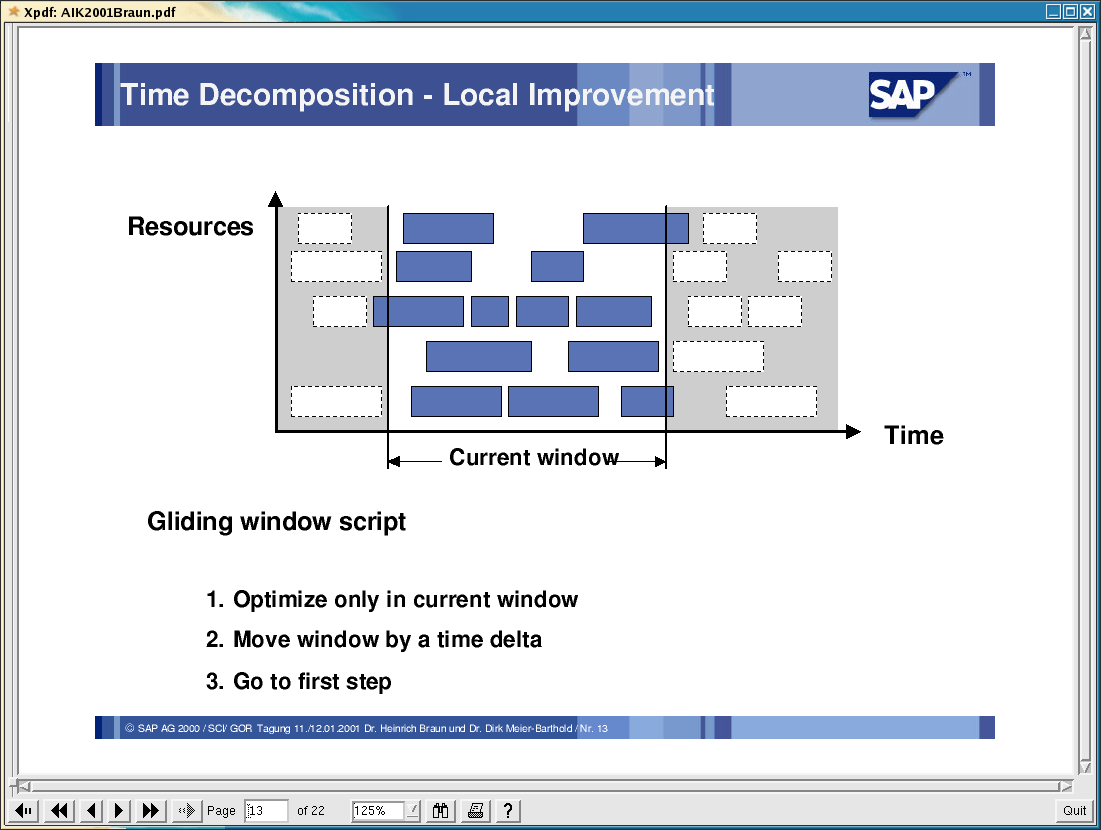
\includegraphics[scale=0.2]{sap1.png} & 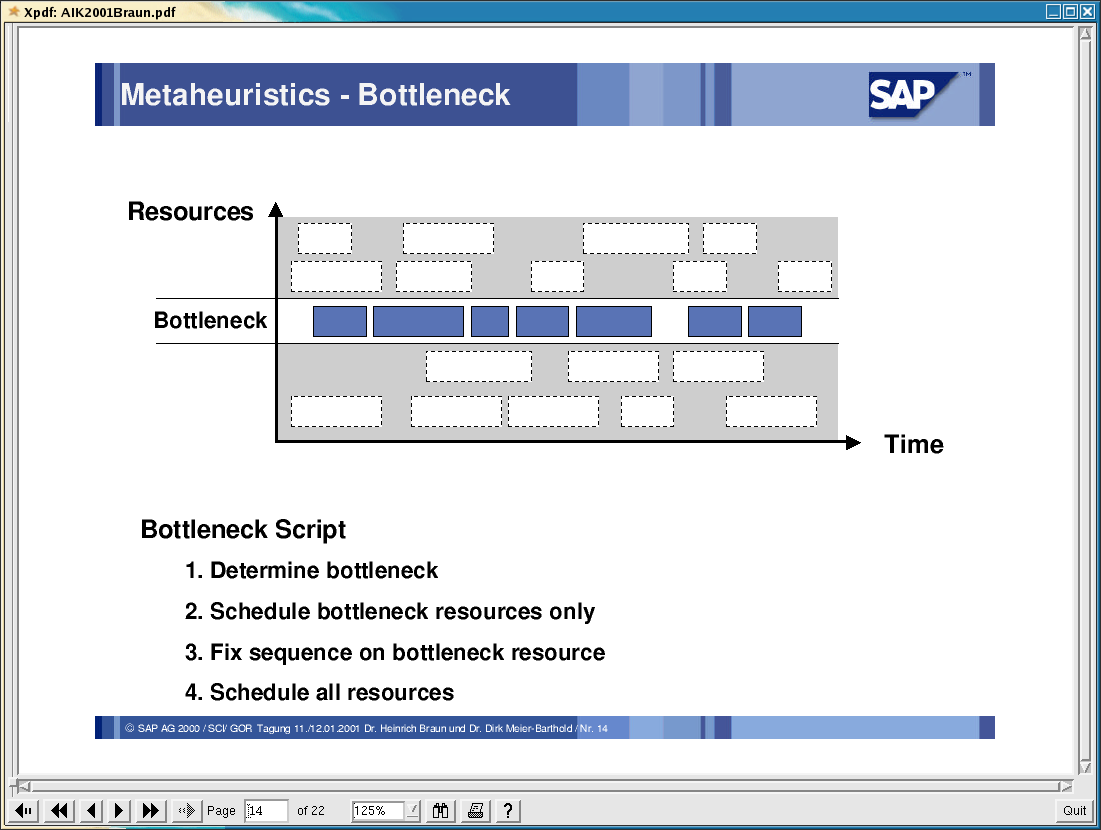
\includegraphics[scale=0.2]{sap2.png}\\
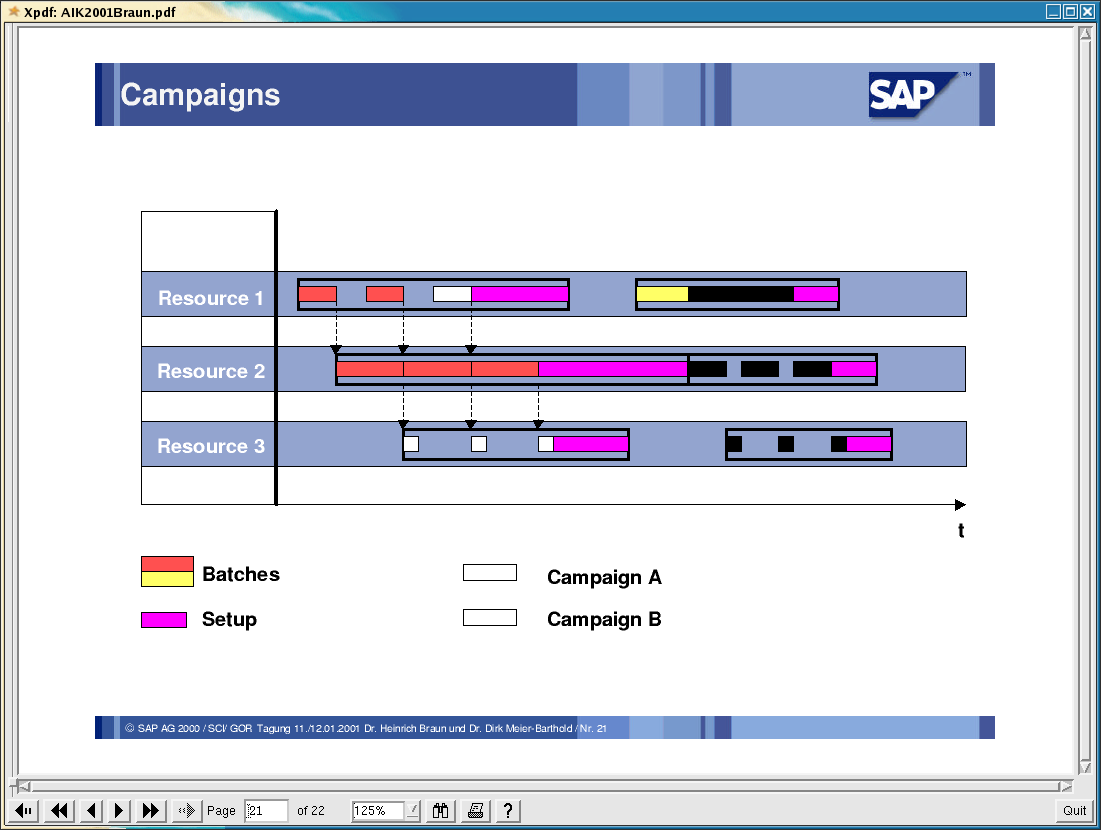
\includegraphics[scale=0.2]{sap3.png} & 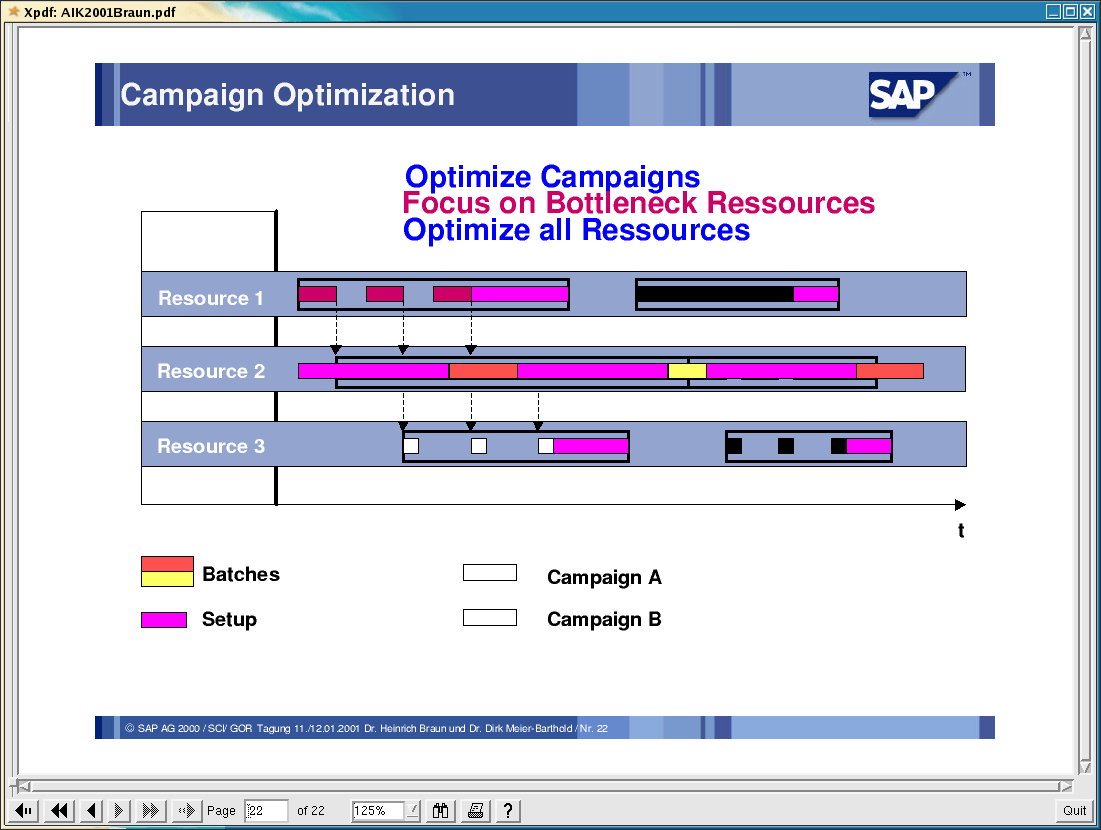
\includegraphics[scale=0.2]{sap4.png}
\end{tabular}
\caption{Optimierer von SAP}
\end{figure}

Oder einem Softwaretool f"ur Strategiespiele:
%\begin{figure}[h]
%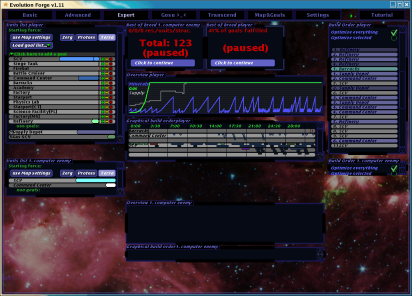
\includegraphics[scale=0.5]{ef.png}
%\caption{Optimierer von Evolution Forge}
%\end{figure}

\begin{thebibliography}{99}
\bibitem{Ross} {\sc Sheldon M. Ross:}  \textit{Introduction to stochastic dynamic programming - Probabilityand mathematical statistics}, First edition, Academic Press, Inc., 1983
\bibitem{SAP} {\sc Dr. Heinrich Braun:}  \textit{Evolution�re Algorithmen im SAP Supply Chain Management}, http://www.aifb.uni-karlsruhe.de/AIK/aik\_07/AIK2001Braun.pdf

\end{thebibliography}
\end{document}

